%!TEX program = xelatex
\documentclass[12pt,a4paper]{exam-zh}

\usepackage{amsmath,array,graphicx,booktabs,multirow}
\usepackage{enumitem}
\usepackage{fancyhdr}
\usepackage{tikz}
\usepackage{tabularx}
\usepackage{setspace}
\setCJKmainfont{Noto Serif CJK SC}
\geometry{margin=2.2cm,top=2.0cm,bottom=2.2cm}
\pagestyle{fancy}
\fancyhf{}
\cfoot{-\thepage{}-}
\renewcommand{\headrulewidth}{0pt}
\renewcommand{\footrulewidth}{0pt}
\setlength{\parindent}{0pt}
\setlength{\parskip}{0.2em}
\setlength{\headheight}{14pt}
\linespread{1.12}
\usepackage{setspace}
\usepackage{eso-pic}
\usetikzlibrary{calc}

%region exam setup

\examsetup{
    page = {
    size = a4paper,           % 设定纸张大小 [4]
    foot-content = { - ; - }  % 页脚显示为 -1-, -2- 格式 [3]
  },
    choices = {
    label-pos = top-left,
    column-sep = 1em,
    label-pos = auto,
    label-sep = 0.5em,
    max-columns = 4
    },
  question = {
    top-sep    = 1em, % 调整题目上方的垂直距离（默认值为 .5em plus .5em minus .2em）
    bottom-sep = 1em  % 调整题目下方的垂直距离（默认值为 .5em plus .5em minus .2em）
  },
    paren = {
    show-paren = false  % 设置为 false 则不显示括号 [3, 4]
  },
    choices = {
    label = \textbf{\Alph*}
  }, 
    solution = {
    show-solution = show-move, % 答案自动移动到卷末
    label-content = {参考答案},  % 答案区的标题文字
    show-qed = true            % 在解答末尾显示结束符号 ◻ 
  }
}

%endregion


%region 卷面变量设置
    % ==========================
    % ==========================
% 卷面变量设置（只需改这里）
% ==========================
\newcommand{\papercode}{SC 05/SC 06}
\newcommand{\examtitle}{2026年金宝培元独立中学八月考}
\newcommand{\examlevel}{高中组}
\newcommand{\examsubject}{高级数学(I)/高级数学}
\newcommand{\sidebartext}{高级数学(I)/一}
\newcommand{\papername}{试卷一}
\newcommand{\papertype}{选择题}
\newcommand{\examdate}{2026年8月7日}
\newcommand{\examtime}{11.00 a.m. 至11.45 a.m.}
\newcommand{\examduration}{45分钟}
\newcommand{\questionpages}{4面}
\newcommand{\paperonepercentage}{40\%}
\newcommand{\papertwopercentage}{60\%}
\newcommand{\setterteacher}{蔡杰庆师}
\newcommand{\reviewteacher}{杨丽芳师}
\newcommand{\auditteacher}{雷泳健师}
    \newcommand{\optrow}[4]{%
    \begin{tabular*}{\linewidth}{@{\extracolsep{\fill}}llll}
    A~#1 & B~#2 & C~#3 & D~#4
    \end{tabular*}%
    }
    \newcommand{\qitem}[5]{\item #1\par\optrow{#2}{#3}{#4}{#5}}
%endregion
    \begin{document}


%region 封面
    \AddToShipoutPictureFG*{%
    \put(31,104){\color{black}\rule{16pt}{66pt}}%
    \put(37,112){\makebox(0,0)[lb]{\rotatebox{90}{\color{white}\bfseries\footnotesize \sidebartext}}}%
    \put(24,18){\makebox(0,0)[lb]{\small 版权所有}}%
    \put(520,18){\makebox(0,0)[lb]{\bfseries\small 【机密】}}%
    }

    \thispagestyle{fancy}

    \begin{minipage}[t]{0.22\linewidth}
    \vspace{0pt}
    \end{minipage}
    \hfill
    \begin{minipage}[t]{0.56\linewidth}
    \centering
    {\zihao{3}\bfseries \examtitle\par}
    \vspace{2.3em}
    {\zihao{3}\bfseries \examlevel\par}
    \vspace{0.3em}
    {\zihao{2}\bfseries \examsubject\par}
    \vspace{0.2em}
    {\large (\papercode)\par}
    \end{minipage}
    \hfill
    \begin{minipage}[t]{0.18\linewidth}
    \vspace{0pt}
    \end{minipage}

    \vspace{3.0em}

    \begin{center}
    \begin{tabular}{c}
        \papername\hspace{2em}\papertype\\[-0.1em]
        \midrule
        日期:\examdate\\[-0.1em]
        时间:\examtime\\[-0.1em]
        (\examduration)\\
        \midrule
    \end{tabular}
    \end{center}

    \vspace{2.0em}

    {\zihao{4}\bfseries \underline{考生须知}\par}
    \vspace{0.8em}

    \begin{enumerate}[label=\arabic*、,leftmargin=2em,itemsep=0.65em]
    \item 本科试卷共分两份：\\
    试卷一：选择题（\paperonepercentage），\\
    试卷二：作答题（\papertwopercentage）。

    \item 考生须于第一阶段规定的60分钟内完成试卷一。第二阶段规定的2小时内作答试卷二。

    \item 试卷一选择题20题全答。选出正确的答案，然后用\textbf{5B铅笔将“O”答案纸}（电脑卡）上相应的字母所在的小方格涂黑。

    \item 可使用电子计算机进行演算。

    \item 试卷一选择题共印\questionpages。
    \end{enumerate}

    \vspace{2.0em}

    \begin{center}
    {\setlength{\fboxrule}{1.2pt}\fbox{\rule{0pt}{1.1em}\hspace{1.2em}{\zihao{4}\bfseries 未经正式宣布\quad 不得翻看内页}\hspace{1.2em}}}
    \end{center}

    \vfill

    \begin{tabular*}{\linewidth}{@{\extracolsep{\fill}}ll}
    考生姓名：\underline{\hspace{4.2cm}} & 考生编号：\underline{\hspace{4.0cm}}
    \end{tabular*}

%endregion

\newpage


%region 范围：高中数学·三角函数 | 考点：三角函数图像的振幅、周期与垂直平移变换 | 难度：中等
\begin{question}
    已知函数 $y = 2\cos 2x + 1$，下列哪一个图像正确表示了该函数在区间 $[-\pi, \pi]$ 上的图像？\paren[C]
    \begin{choices}
        \item
        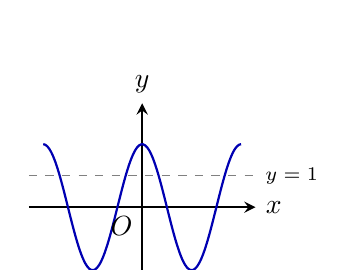
\begin{tikzpicture}[scale=0.4, >=stealth, baseline]
            \draw[->, thick] (-3.6, 0) -- (3.6, 0) node[right] {$x$};
            \draw[->, thick] (0, -2.3) -- (0, 3.3) node[above] {$y$};
            \draw[dashed, gray] (-3.6, 1) -- (3.6, 1);
            \draw[domain=-3.14159:3.14159, smooth, samples=100, thick, blue!70!black]
                plot (\x, {2*cos(2*\x r)});
            \node[below left] at (0,0) {$O$};
            \node[right] at (3.6, 1) {\scriptsize $y=1$};
        \end{tikzpicture}

        \item
        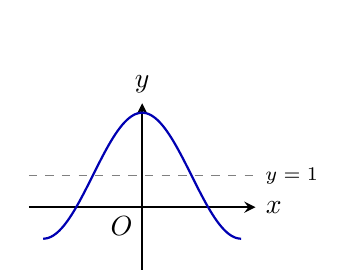
\begin{tikzpicture}[scale=0.4, >=stealth, baseline]
            \draw[->, thick] (-3.6, 0) -- (3.6, 0) node[right] {$x$};
            \draw[->, thick] (0, -2.3) -- (0, 3.3) node[above] {$y$};
            \draw[dashed, gray] (-3.6, 1) -- (3.6, 1);
            \draw[domain=-3.14159:3.14159, smooth, samples=100, thick, blue!70!black]
                plot (\x, {2*cos(\x r) + 1});
            \node[below left] at (0,0) {$O$};
            \node[right] at (3.6, 1) {\scriptsize $y=1$};
        \end{tikzpicture}

        \item
        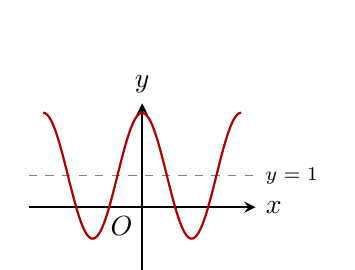
\begin{tikzpicture}[scale=0.4, >=stealth, baseline]
            \draw[->, thick] (-3.6, 0) -- (3.6, 0) node[right] {$x$};
            \draw[->, thick] (0, -2.3) -- (0, 3.3) node[above] {$y$};
            \draw[dashed, gray] (-3.6, 1) -- (3.6, 1);
            \draw[domain=-3.14159:3.14159, smooth, samples=100, thick, red!70!black]
                plot (\x, {2*cos(2*\x r) + 1});
            \node[below left] at (0,0) {$O$};
            \node[right] at (3.6, 1) {\scriptsize $y=1$};
        \end{tikzpicture}

        \item
        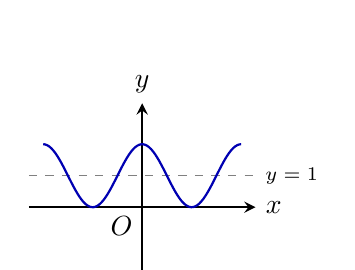
\begin{tikzpicture}[scale=0.4, >=stealth, baseline]
            \draw[->, thick] (-3.6, 0) -- (3.6, 0) node[right] {$x$};
            \draw[->, thick] (0, -2.3) -- (0, 3.3) node[above] {$y$};
            \draw[dashed, gray] (-3.6, 1) -- (3.6, 1);
            \draw[domain=-3.14159:3.14159, smooth, samples=100, thick, blue!70!black]
                plot (\x, {cos(2*\x r) + 1});
            \node[below left] at (0,0) {$O$};
            \node[right] at (3.6, 1) {\scriptsize $y=1$};
        \end{tikzpicture}
    \end{choices}
\end{question}

\begin{solution}
    \textbf{解析：} \\
    函数 $y = 2\cos 2x + 1$ 可视为由基本函数 $y = \cos x$ 经过三次变换叠加而成，需逐一核对各选项是否同时满足这三项特征：

    \textbf{特征一（振幅）：} 系数 $2$ 使振幅由 $1$ 变为 $2$，图像应在 $y$ 方向上下界之间来回摆动，最大值与最小值之间的振动幅度须为 $2$（而非 $1$）。选项 (A) 中曲线波动幅度过小，振幅明显只有 $1$，不符合，可排除。

    \textbf{特征二（周期）：} 角度部分为 $2x$，故周期为
    \[ \displaystyle T = \frac{2\pi}{2} = \pi \]
    图像应在 $[-\pi, \pi]$ 区间内完整呈现两个周期。选项 (B) 与选项 (D) 中曲线在同一区间内仅呈现一个完整周期，说明其周期仍为 $2\pi$，即角度部分未乘以 $2$，因此可排除。

    \textbf{特征三（垂直平移）：} 常数项 $+1$ 使图像整体向上平移 $1$ 个单位，函数的中心线（振动中心）应为直线 $y=1$，而非 $y=0$。选项 (A) 的图像以 $x$ 轴为振动中心，未体现向上平移，故进一步确认其错误。

    综合以上三项特征——振幅为 $2$、周期为 $\pi$、图像沿 $y=1$ 上下振动——只有选项 (C) 同时满足。

    故选 C。
\end{solution}
%endregion

%region 范围：高中数学·三角函数 | 考点：诱导公式与象限角三角函数值符号判断 | 难度：中等
\begin{question}
    已知 $\theta$ 为第三象限角，且 $\cos\theta = a$，求 $\cos\left(\theta + \dfrac{5\pi}{2}\right)$ 的值（用 $a$ 表示）。\paren[B]
    \begin{choices}
        \item $-\sqrt{1-a^2}$
        \item $\sqrt{1-a^2}$
        \item $-a$
        \item $a$
    \end{choices}
\end{question}

\begin{solution}
    \textbf{解析：} \\
    首先将角 $\theta + \dfrac{5\pi}{2}$ 化为周期内的等价角，以便应用诱导公式。注意到
    \[ \displaystyle \frac{5\pi}{2} = 2\pi + \frac{\pi}{2} \]
    由余弦函数以 $2\pi$ 为周期，可知
    \[ \displaystyle \cos\left(\theta + \frac{5\pi}{2}\right) = \cos\left(\theta + \frac{\pi}{2}\right) \]

    接下来应用诱导公式 $\cos\left(\theta + \dfrac{\pi}{2}\right) = -\sin\theta$，故
    \[ \displaystyle \cos\left(\theta + \frac{5\pi}{2}\right) = -\sin\theta \]

    由于 $\theta$ 是第三象限角，该象限内正弦值为负，即 $\sin\theta < 0$。结合同角关系 $\sin^2\theta + \cos^2\theta = 1$ 及 $\cos\theta = a$，可得
    \[ \displaystyle \sin\theta = -\sqrt{1-a^2} \]

    代入前式：
    \[ \displaystyle \cos\left(\theta + \frac{5\pi}{2}\right) = -\sin\theta = -\left(-\sqrt{1-a^2}\right) = \sqrt{1-a^2} \]

    选项 (A) 混淆了 $\sin\theta$ 本身的符号与诱导公式中负号叠加后的最终结果，误将两次负号只算了一次；选项 (C) 与 (D) 则是错误地将 $\dfrac{5\pi}{2}$ 当作 $\pi$ 的诱导公式处理（误用 $\cos(\theta+\pi) = -\cos\theta$ 型公式），未能正确化简角度，属于诱导公式选用错误。

    故选 B。
\end{solution}
%endregion

%region 范围：高中数学·解三角形 | 考点：余弦定理逆用——由三边比例判断最大角 | 难度：中等
\begin{question}
    在 $\triangle ABC$ 中，三边长之比为 $a : b : c = 1 : \sqrt{3} : \sqrt{7}$。求该三角形中最长边所对的角。\paren[C]
    \begin{choices}
        \item $90°$
        \item $120°$
        \item $150°$
        \item $135°$
    \end{choices}
\end{question}

\begin{solution}
    \textbf{解析：} \\
    由三角形中"大边对大角"的性质可知，比例中数值最大的边 $c$（对应比例系数 $\sqrt{7}$）所对的角 $C$ 即为最大角。因为比例系数在余弦定理计算中可直接约去，故可直接用比例值 $a=1,\ b=\sqrt{3},\ c=\sqrt{7}$ 代入余弦定理的逆用形式：
    \[ \displaystyle \cos C = \frac{a^2 + b^2 - c^2}{2ab} \]

    代入数值：
    \[ \displaystyle \cos C = \frac{1^2 + (\sqrt{3})^2 - (\sqrt{7})^2}{2 \times 1 \times \sqrt{3}} = \frac{1 + 3 - 7}{2\sqrt{3}} = \frac{-3}{2\sqrt{3}} \]

    分母有理化：
    \[ \displaystyle \cos C = \frac{-3}{2\sqrt{3}} = \frac{-3\sqrt{3}}{6} = -\frac{\sqrt{3}}{2} \]

    由 $\cos C = -\dfrac{\sqrt{3}}{2}$ 且 $C \in (0°, 180°)$，可得
    \[ \displaystyle C = 150° \]

    选项 (A) 是误判 $\cos C = 0$ 对应的直角，忽视了计算出的负值结果；选项 (B) 是把 $\cos C = -\dfrac{\sqrt3}{2}$ 误记为 $-\dfrac12$ 所对应的特殊角，属于特殊角三角函数值记混；选项 (D) 则是误记为 $-\dfrac{\sqrt2}{2}$ 对应的角度，同样属于特殊角余弦值混淆。

    故选 C。
\end{solution}
%endregion

%region 范围：高中数学·解三角形 | 考点：三角形面积公式反推夹角与余弦定理求第三边（两解取舍） | 难度：中等偏难
\begin{question}
    在 $\triangle ABC$ 中，已知 $a = 4$，$b = 5$，且 $\triangle ABC$ 的面积为 $5\sqrt{3}$。若已知该三角形为钝角三角形，求第三边 $c$ 的长度。\paren[B]
    \begin{choices}
        \item $\sqrt{21}$
        \item $\sqrt{61}$
        \item $\sqrt{41}$
        \item $9$
    \end{choices}
\end{question}

\begin{solution}
    \textbf{解析：} \\
    已知两边 $a$、$b$ 及三角形面积，应先利用面积公式反求夹角 $C$（即 $a$、$b$ 两边的夹角）：
    \[ \displaystyle S = \frac{1}{2}ab\sin C \]

    代入 $a=4$，$b=5$，$S=5\sqrt{3}$：
    \[ \displaystyle 5\sqrt{3} = \frac{1}{2}(4)(5)\sin C = 10\sin C \]
    \[ \displaystyle \sin C = \frac{5\sqrt{3}}{10} = \frac{\sqrt{3}}{2} \]

    由 $\sin C = \dfrac{\sqrt3}{2}$ 且 $C \in (0°, 180°)$，可知 $C$ 存在两个可能取值：
    \[ \displaystyle C = 60° \quad \text{或} \quad C = 120° \]

    这是本题的关键陷阱：仅由 $\sin C$ 的值无法唯一确定角 $C$，必须结合题目补充条件"该三角形为钝角三角形"进行取舍。由于 $a=4$、$b=5$ 均为已知边，若 $C=60°$（锐角），还需验证三角形是否可能在别处存在钝角；但由三角形内角和及边长关系可知，此时最大边所对角才可能为钝角，而 $C$ 是唯一可能达到钝角数值的角（因为 $\sin C$ 相同但 $\cos C$ 符号相反）。结合题目已直接给出三角形为钝角三角形，可确定应取：
    \[ \displaystyle C = 120° \]

    利用余弦定理求 $c$：
    \[ \displaystyle c^2 = a^2 + b^2 - 2ab\cos C = 4^2 + 5^2 - 2(4)(5)\cos 120° \]
    \[ \displaystyle c^2 = 16 + 25 - 40 \times \left(-\frac{1}{2}\right) = 41 + 20 = 61 \]
    \[ \displaystyle c = \sqrt{61} \]

    选项 (A) 是误取了 $C=60°$（锐角）代入余弦定理所得的结果，忽视了题目"钝角三角形"这一限定条件，属于两解取舍错误；选项 (C) 是在计算 $2ab\cos C$ 时正负号处理错误，将其误算为加法而非减去负值的形式；选项 (D) 则是脱离余弦定理，直接对边长做简单估算，未经过正确的公式运算。

    故选 B。
\end{solution}
%endregion


%region 范围：高中数学-二倍角公式与三角函数最值 | 考点：提取公因式后连续运用二倍角公式化简求最值 | 难度：基础
\begin{question}
    求函数 $f(\theta) = 2\left(\sin\theta\cos^3\theta - \sin^3\theta\cos\theta\right)$ 的最大值。 \paren[B]
    \begin{choices}
        \item $\dfrac{1}{4}$
        \item $\dfrac{1}{2}$
        \item $1$
        \item $2$
    \end{choices}
\end{question}

\begin{solution}
    求 $f(\theta) = 2\left(\sin\theta\cos^3\theta - \sin^3\theta\cos\theta\right)$ 的最大值。 \\
    先提取公因式化简，再连续运用二倍角公式。
    \begin{align*}
        f(\theta) &= 2\sin\theta\cos\theta\left(\cos^2\theta-\sin^2\theta\right) \\
        &= \sin2\theta \cdot \cos2\theta \\
        &= \frac{1}{2}\sin4\theta
    \end{align*}
    当 $\sin4\theta = 1$ 时，$f(\theta)$ 取得最大值 $\dfrac{1}{2}$。 \\
    故选 B。
\end{solution}
%endregion
% %region 范围：高中数学·三角恒等变换 | 考点：三倍角公式展开与二倍角公式化简求最值 | 难度：中等偏难
% \begin{question}
%     求函数 $f(\theta) = 2\sin\theta\cos^3\theta - \sin3\theta\cos\theta$ 的最大值。\paren[A]
%     \begin{choices}
%         \item $\dfrac{1}{4}$
%         \item $\dfrac{1}{2}$
%         \item $1$
%         \item $-\dfrac{1}{4}$
%     \end{choices}
% \end{question}

% \begin{solution}
%     \textbf{解析：} \\
%     先利用三倍角公式 $\sin3\theta = 3\sin\theta - 4\sin^3\theta$ 将 $\sin3\theta\cos\theta$ 展开，代入原式：
%     \[ \displaystyle f(\theta) = 2\sin\theta\cos^3\theta - (3\sin\theta - 4\sin^3\theta)\cos\theta \]
%     \[ \displaystyle = 2\sin\theta\cos^3\theta - 3\sin\theta\cos\theta + 4\sin^3\theta\cos\theta \]

%     提取公因式 $\sin\theta\cos\theta$：
%     \[ \displaystyle f(\theta) = \sin\theta\cos\theta\left(2\cos^2\theta - 3 + 4\sin^2\theta\right) \]

%     利用同角关系 $\cos^2\theta = 1 - \sin^2\theta$ 将括号内式子统一为 $\sin^2\theta$ 的表达式：
%     \[ \displaystyle 2\cos^2\theta - 3 + 4\sin^2\theta = 2(1-\sin^2\theta) - 3 + 4\sin^2\theta = -1 + 2\sin^2\theta \]

%     再利用二倍角公式 $\cos2\theta = 1 - 2\sin^2\theta$，可知 $-1+2\sin^2\theta = -\cos2\theta$，故
%     \[ \displaystyle f(\theta) = \sin\theta\cos\theta \cdot (-\cos2\theta) = -\sin\theta\cos\theta\cos2\theta \]

%     再次利用二倍角公式 $\sin\theta\cos\theta = \dfrac{1}{2}\sin2\theta$，代入：
%     \[ \displaystyle f(\theta) = -\frac{1}{2}\sin2\theta\cos2\theta = -\frac{1}{4}\sin4\theta \]

%     （此处再次运用二倍角公式 $\sin2\theta\cos2\theta = \dfrac{1}{2}\sin4\theta$。）

%     由于 $\sin4\theta \in [-1, 1]$，当 $\sin4\theta = -1$ 时，$f(\theta)$ 取得最大值：
%     \[ \displaystyle f(\theta)_{\max} = -\frac{1}{4} \times (-1) = \frac{1}{4} \]

%     选项 (B) 是漏做了最后一步 $\sin2\theta\cos2\theta = \dfrac12\sin4\theta$ 的二倍角合并，误将 $-\dfrac12\sin4\theta$ 本身的振幅当作答案；选项 (C) 是同时漏掉了两次二倍角合并中的系数 $\dfrac12$，把振幅误算为 $1$；选项 (D) 则是符号判断错误，误取 $\sin4\theta=1$ 时的函数值作为最大值，实际上那对应的是函数的最小值。

%     故选 A。
% \end{solution}
% %endregion

%region 范围：高中数学·三角方程 | 考点：三角方程求解——因式分解法与两边同除丢根陷阱 | 难度：中等
\begin{question}
    求方程 $\tan x = 2\sin x$ 在区间 $[0, 2\pi)$ 内解的个数。\paren[C]
    \begin{choices}
        \item $2$
        \item $3$
        \item $4$
        \item $6$
    \end{choices}
\end{question}

\begin{solution}
    \textbf{解析：} \\
    将 $\tan x = \dfrac{\sin x}{\cos x}$ 代入原方程（注意 $\cos x \neq 0$，即 $x \neq \dfrac{\pi}{2}, \dfrac{3\pi}{2}$）：
    \[ \displaystyle \frac{\sin x}{\cos x} = 2\sin x \]

    将等式两边同乘以 $\cos x$（而非直接两边同除以 $\sin x$，以避免遗漏 $\sin x = 0$ 的解），移项整理：
    \[ \displaystyle \sin x = 2\sin x\cos x \]
    \[ \displaystyle \sin x - 2\sin x\cos x = 0 \]

    提取公因式 $\sin x$：
    \[ \displaystyle \sin x\,(1 - 2\cos x) = 0 \]

    因此原方程等价于两种情况：$\sin x = 0$ 或 $\cos x = \dfrac{1}{2}$，需分别求解并检验是否落在 $\cos x \neq 0$ 的定义域内。

    \textbf{情况一：$\sin x = 0$} \\
    在 $[0, 2\pi)$ 内，$\sin x = 0$ 的解为 $x = 0$ 或 $x = \pi$。经检验，此时 $\cos x = 1$ 或 $\cos x = -1$，均满足 $\cos x \neq 0$，故两解均成立。

    \textbf{情况二：$\cos x = \dfrac{1}{2}$} \\
    在 $[0, 2\pi)$ 内，解得 $x = \dfrac{\pi}{3}$ 或 $x = \dfrac{5\pi}{3}$，显然满足 $\cos x \neq 0$，故两解均成立。

    综合两种情况，方程在 $[0, 2\pi)$ 内共有 $4$ 个解：$x = 0,\ \dfrac{\pi}{3},\ \pi,\ \dfrac{5\pi}{3}$。

    选项 (A) 是错误地将两边直接除以 $\sin x$（默认 $\sin x \neq 0$），从而遗漏了 $\sin x = 0$ 对应的两个解，只保留了 $\cos x = \dfrac12$ 的解；选项 (B) 是遗漏了 $\sin x=0$ 情况中的 $x=0$（可能误认为区间为开区间 $(0,2\pi)$ 而排除端点）；选项 (D) 则是误将 $\cos x=\dfrac12$ 求解时同时把 $\pm\dfrac{\pi}{3}$ 及其周期延伸的角度都计入，重复计数导致解的个数虚增。

    故选 C。
\end{solution}
%endregion

\newpage


%region 范围：高中数学-直线方程与斜率 | 考点：由直线一般式求斜率、点在直线上代入求参数 | 难度：中等
\begin{question}
    已知直线 $ax+by=2$ 的斜率为 $-\dfrac{1}{2}$，且经过点 $(4,1)$，求 $a+b$ 的值。 \paren[B]
    \begin{choices}
        \item $-1$
        \item $1$
        \item $\dfrac{2}{3}$
        \item $2$
    \end{choices}
\end{question}

\begin{solution}
    已知直线 $ax+by=2$ 的斜率为 $-\dfrac{1}{2}$，且经过点 $(4,1)$，求 $a+b$。 \\
    将直线化为斜截式求出斜率与 $a,b$ 的关系，再代入点坐标联立求解。
    \begin{align*}
        ax+by &= 2 \\
        y &= -\frac{a}{b}x+\frac{2}{b}
    \end{align*}
    由斜率条件 $-\dfrac{a}{b}=-\dfrac{1}{2}$，得 $a=\dfrac{b}{2}$。 \\
    代入点 $(4,1)$：
    \begin{align*}
        a(4)+b(1) &= 2 \\
        \frac{b}{2}(4)+b &= 2 \\
        2b+b &= 2 \\
        3b &= 2
    \end{align*}
    解得 $b=\dfrac{2}{3}$，$a=\dfrac{1}{3}$。
    \[
        a+b = \frac{1}{3}+\frac{2}{3} = 1
    \]
    故选 B。
\end{solution}
%endregion
% %region 范围：高中数学·直线与圆·距离公式 | 考点：由两定点距离之比求动点轨迹方程（阿波罗尼奥斯圆） | 难度：中等偏难
% \begin{question}
%     已知平面上两定点 $A(-1, 0)$ 与 $B(2, 0)$，动点 $P(x, y)$ 满足 $|PA| : |PB| = 1 : 2$，求点 $P$ 的轨迹方程。\paren[B]
%     \begin{choices}
%         \item $(x-2)^2 + y^2 = 4$
%         \item $(x+2)^2 + y^2 = 4$
%         \item $(x+2)^2 + y^2 = 16$
%         \item $(x-\frac{1}{3})^2 + y^2 = \frac{4}{3}$
%     \end{choices}
% \end{question}

% \begin{solution}
%     \textbf{解析：} \\
%     设动点 $P(x, y)$，由距离公式分别写出 $|PA|^2$ 与 $|PB|^2$：
%     \[ \displaystyle |PA|^2 = (x+1)^2 + y^2, \qquad |PB|^2 = (x-2)^2 + y^2 \]

%     由条件 $|PA| : |PB| = 1 : 2$，即 $|PB| = 2|PA|$，两边平方（避免根号，直接用距离平方之比处理）：
%     \[ \displaystyle |PB|^2 = 4|PA|^2 \]

%     代入并展开：
%     \[ \displaystyle (x-2)^2 + y^2 = 4\left[(x+1)^2 + y^2\right] \]
%     \[ \displaystyle x^2 - 4x + 4 + y^2 = 4x^2 + 8x + 4 + 4y^2 \]

%     移项整理，将所有项集中到等式一侧：
%     \[ \displaystyle x^2 - 4x + 4 + y^2 - 4x^2 - 8x - 4 - 4y^2 = 0 \]
%     \[ \displaystyle -3x^2 - 12x - 3y^2 = 0 \]

%     两边同除以 $-3$：
%     \[ \displaystyle x^2 + 4x + y^2 = 0 \]

%     对 $x$ 项配方：
%     \[ \displaystyle (x^2 + 4x + 4) + y^2 = 4 \]
%     \[ \displaystyle (x+2)^2 + y^2 = 4 \]

%     因此点 $P$ 的轨迹是以 $(-2, 0)$ 为圆心、半径为 $2$ 的圆。

%     选项 (A) 是把比值方向搞反，误设为 $|PA| = 2|PB|$（即误解为 $|PA|:|PB|=2:1$），导致配方后圆心落在 $B$ 一侧的 $(2,0)$；选项 (C) 是配方时半径计算错误，把 $4$ 误写为常数项 $16$，忽略了配方补齐的系数关系；选项 (D) 则是在两边平方或移项过程中系数处理错误，未能正确合并 $x^2$ 项系数，导致圆心与半径均计算失真。

%     故选 B。
% \end{solution}
% %endregion

%region 范围：高中数学·平面向量与坐标几何 | 考点：外分点公式的应用与内分/外分公式混淆辨析 | 难度：中等偏难
\begin{question}
    已知两点 $A(a, 2)$ 与 $B(4, b)$。若点 $C(10, -1)$ 是线段 $AB$ 延长线上的外分点，且满足 $AC : CB = 3 : 1$，求 $a + b$ 的值。\paren[A]
    \begin{choices}
        \item $-8$
        \item $4$
        \item $-4$
        \item $8$
    \end{choices}
\end{question}

\begin{solution}
    \textbf{解析：} \\
    外分点公式与内分点公式形式相近但符号不同，需特别注意区分。若点 $C$ 是线段 $AB$ 的外分点，且 $AC : CB = m : n$（$m \neq n$），则
    \[ \displaystyle C = \left( \frac{mB_x - nA_x}{m - n},\ \frac{mB_y - nA_y}{m - n} \right) \]
    （与内分点公式 $\dfrac{nA+mB}{m+n}$ 相比，外分点公式的分母为 $m-n$，且其中一项带负号，这正是外分与内分的本质区别。）

    本题中 $m=3$，$n=1$，$A=(a,2)$，$B=(4,b)$，$C=(10,-1)$，代入公式分别列出 $x$、$y$ 坐标方程：

    \textbf{求 $x$ 坐标方程：}
    \[ \displaystyle 10 = \frac{3(4) - 1(a)}{3 - 1} = \frac{12 - a}{2} \]
    \[ \displaystyle 20 = 12 - a \implies a = 12 - 20 = -8 \]

    \textbf{求 $y$ 坐标方程：}
    \[ \displaystyle -1 = \frac{3(b) - 1(2)}{3 - 1} = \frac{3b - 2}{2} \]
    \[ \displaystyle -2 = 3b - 2 \implies 3b = 0 \implies b = 0 \]

    因此：
    \[ \displaystyle a + b = -8 + 0 = -8 \]

    选项 (B) 是误用内分点公式 $\dfrac{nA+mB}{m+n}$ 代替外分点公式进行计算，混淆了内分与外分的本质区别；选项 (C) 是外分点公式中 $m$、$n$ 的位置颠倒（即误将 $AC:CB=3:1$ 当作 $AC:CB=1:3$ 代入），导致符号与数值均出现偏差；选项 (D) 则是在化简 $\dfrac{12-a}{2}=10$ 与 $\dfrac{3b-2}{2}=-1$ 的过程中，误将分子中的减号看作加号，导致 $a$、$b$ 的正负号计算错误。

    故选 A。
\end{solution}
%endregion


%region 范围：高中数学·平面直角坐标系与多边形面积 | 考点：鞋带公式应用——顶点连接顺序的判断与重新排列 | 难度：困难
\begin{question}
    在平面直角坐标系中，四边形的四个顶点坐标分别为 $M(1, 5)$、$N(-2, -3)$、$P(-3, 2)$、$Q(3, -1)$。求该四边形的面积。\paren[A]
    \begin{choices}
        \item $28.5$
        \item $3.5$
        \item $57$
        \item $14.5$
    \end{choices}
\end{question}

\begin{solution}
    \textbf{解析：} \\
    鞋带公式要求将顶点按其在平面上实际相连的顺序（顺时针或逆时针）依次代入，若直接按题目给出的标号顺序代入而不加辨别，很可能得到自相交（蝴蝶形）四边形对应的错误"面积"。因此第一步必须先确定四点的正确连接顺序。

    将四点坐标标于坐标系中可知：$M(1,5)$ 位于右上方，$P(-3,2)$ 位于左侧，$N(-2,-3)$ 位于左下方，$Q(3,-1)$ 位于右下方。按逆时针方向排列，四点的正确连接顺序应为
    \[ \displaystyle M \to P \to N \to Q \to M \]

    按此正确顺序代入鞋带公式：
    \[ \displaystyle S = \frac{1}{2}\left|(x_My_P+x_Py_N+x_Ny_Q+x_Qy_M)-(y_Mx_P+y_Px_N+y_Nx_Q+y_Qx_M)\right| \]

    \textbf{正向乘积之和：}
    \[ \displaystyle (1)(2)+(-3)(-3)+(-2)(-1)+(3)(5) = 2+9+2+15 = 28 \]

    \textbf{反向乘积之和：}
    \[ \displaystyle (5)(-3)+(2)(-2)+(-3)(3)+(-1)(1) = -15-4-9-1 = -29 \]

    代入公式：
    \[ \displaystyle S = \frac{1}{2}\left|28-(-29)\right| = \frac{1}{2}\times 57 = 28.5 \]

    选项 (B) 是未经判断，直接按题目给出的标号顺序 $M \to N \to P \to Q$（并非实际连接顺序）盲目代入鞋带公式，得到的是自相交四边形对应的错误结果 $3.5$，这正是本题设置"顺序未按连接顺序排列"这一条件所要考察的核心陷阱；选项 (C) 是在使用正确连接顺序算出正向与反向乘积之和后，忘记乘以公式最外层的 $\dfrac12$，直接把 $57$ 当作面积；选项 (D) 则是只计算了反向乘积之和的绝对值再取一半（即 $\dfrac12|-29|=14.5$），遗漏了正向乘积部分的运算。

    故选 A。
\end{solution}
%endregion

%region 范围：高中/大学预备微积分·微分的应用 | 考点：隐函数求导法求曲线切线斜率 | 难度：中等偏难
\begin{question}
    已知曲线方程为 $x^3 + xy + y^3 = 3$，求该曲线在 $x = 1$ 处的切线斜率。\paren[C]
    \begin{choices}
        \item $-7$
        \item $-\dfrac{3}{4}$
        \item $-1$
        \item $\dfrac{3}{4}$
    \end{choices}
\end{question}

\begin{solution}
    \textbf{解析：} \\
    首先需确定 $x=1$ 时对应的 $y$ 值。将 $x=1$ 代入原方程：
    \[ \displaystyle 1 + y + y^3 = 3 \implies y^3 + y - 2 = 0 \]
    因式分解：$(y-1)(y^2+y+2) = 0$。由于 $y^2+y+2=0$ 的判别式为负（无实数解），故唯一实数解为
    \[ \displaystyle y = 1 \]
    即所求切点为 $(1, 1)$。

    由于 $y$ 是 $x$ 的隐函数，须对方程两边同时对 $x$ 求导，其中 $xy$ 项须使用\textbf{乘积法则}，$y^3$ 项须使用\textbf{链式法则}：
    \[ \displaystyle \frac{d}{dx}(x^3) + \frac{d}{dx}(xy) + \frac{d}{dx}(y^3) = \frac{d}{dx}(3) \]
    \[ \displaystyle 3x^2 + \left(y + x\frac{dy}{dx}\right) + 3y^2\frac{dy}{dx} = 0 \]

    将含 $\dfrac{dy}{dx}$ 的项移至一侧并提取公因式：
    \[ \displaystyle \frac{dy}{dx}\left(x + 3y^2\right) = -\left(3x^2 + y\right) \]
    \[ \displaystyle \frac{dy}{dx} = \frac{-(3x^2+y)}{x+3y^2} \]

    代入切点坐标 $x=1$，$y=1$：
    \[ \displaystyle \frac{dy}{dx} = \frac{-(3(1)^2+1)}{1+3(1)^2} = \frac{-(3+1)}{1+3} = \frac{-4}{4} = -1 \]

    选项 (A) 是对 $y^3$ 项求导时遗漏了链式法则中的 $\dfrac{dy}{dx}$ 因子，误将其求导结果当作 $3y^2$（视为常数处理），导致该项未能移到含 $\dfrac{dy}{dx}$ 的一侧参与合并，从而计算出错误结果 $-7$；选项 (B) 与 (D) 是对 $xy$ 项求导时遗漏了乘积法则中的 $y$ 这一项，误将 $\dfrac{d}{dx}(xy)$ 直接写成 $x\dfrac{dy}{dx}$（漏掉 $+y$），(D) further 在最后一步符号处理上出现正负号颠倒。

    故选 C。
\end{solution}
%endregion

%region 范围：高中/大学预备微积分·导数的应用 | 考点：利用二阶导数判别法求函数极大值 | 难度：中等
\begin{question}
    已知函数 $f(x) = x + \dfrac{4}{x}$（$x \neq 0$），求 $f(x)$ 的极大值。\paren[D]
    \begin{choices}
        \item $4$
        \item $-2$
        \item $2$
        \item $-4$
    \end{choices}
\end{question}

\begin{solution}
    \textbf{解析：} \\
    先对 $f(x)$ 求一阶导数，寻找可能的极值点（驻点）：
    \[ \displaystyle f'(x) = 1 - \frac{4}{x^2} \]

    令 $f'(x) = 0$：
    \[ \displaystyle 1 - \frac{4}{x^2} = 0 \implies x^2 = 4 \implies x = 2 \ \text{或} \ x = -2 \]

    由于本题存在两个驻点，仅求出驻点并不能确定哪一个对应极大值，必须进一步用二阶导数判别法逐一检验，这正是本题容易出错的关键步骤。求二阶导数：
    \[ \displaystyle f''(x) = \frac{8}{x^3} \]

    \textbf{检验 $x = 2$：}
    \[ \displaystyle f''(2) = \frac{8}{2^3} = \frac{8}{8} = 1 > 0 \]
    二阶导数为正，故 $x=2$ 是极小值点，对应极小值 $f(2) = 2 + \dfrac{4}{2} = 4$（并非本题所求）。

    \textbf{检验 $x = -2$：}
    \[ \displaystyle f''(-2) = \frac{8}{(-2)^3} = \frac{8}{-8} = -1 < 0 \]
    二阶导数为负，故 $x=-2$ 才是极大值点。代入求极大值：
    \[ \displaystyle f(-2) = -2 + \frac{4}{-2} = -2 - 2 = -4 \]

    因此，$f(x)$ 的极大值为 $-4$（在 $x=-2$ 处取得）。

    选项 (A) 是把极小值点 $x=2$ 处的函数值 $4$ 误当作极大值，属于混淆极大值点与极小值点的典型错误；选项 (B) 是仅求出驻点 $x=-2$ 后未代回原函数计算，直接把 $x$ 坐标本身当作极值；选项 (C) 则是同样把驻点 $x=2$ 的横坐标误当作纵坐标（极值）。

    故选 D。
\end{solution}
%endregion

%region 范围：高中/大学预备微积分·相关变化率 | 考点：链式法则求面积随时间的变化率 | 难度：中等
\begin{question}
    一圆形薄片的半径以 $2\text{ cm/s}$ 的速率减少。当该圆的直径为 $20\text{ cm}$ 时，求其面积改变的速率。\paren[B]
    \begin{choices}
        \item $-80\pi \text{ cm}^2/\text{s}$
        \item $-40\pi \text{ cm}^2/\text{s}$
        \item $-20\pi \text{ cm}^2/\text{s}$
        \item $40\pi \text{ cm}^2/\text{s}$
    \end{choices}
\end{question}

\begin{solution}
    \textbf{解析：} \\
    设圆的半径为 $r$（单位：cm），面积为 $A$（单位：$\text{cm}^2$），则
    \[ \displaystyle A = \pi r^2 \]

    由于半径以 $2\text{ cm/s}$ 的速率\textbf{减少}，故 $\dfrac{dr}{dt} = -2\text{ cm/s}$（负号表示半径随时间递减，这是本题容易遗漏的符号细节）。

    利用链式法则，将 $A$ 对时间 $t$ 求导（注意 $A$ 是 $r$ 的函数，$r$ 又是 $t$ 的函数）：
    \[ \displaystyle \frac{dA}{dt} = \frac{dA}{dr}\cdot\frac{dr}{dt} = 2\pi r \cdot \frac{dr}{dt} \]

    题目给出的是直径为 $20\text{ cm}$，须先换算为半径，这是另一处容易出错的关键：
    \[ \displaystyle r = \frac{20}{2} = 10 \text{ cm} \]

    代入 $r=10$，$\dfrac{dr}{dt}=-2$：
    \[ \displaystyle \frac{dA}{dt} = 2\pi(10)(-2) = -40\pi \ \text{cm}^2/\text{s} \]

    即该圆的面积正以 $40\pi\text{ cm}^2/\text{s}$ 的速率\textbf{减少}。

    选项 (A) 是误将题目给出的直径 $20$ 直接当作半径代入公式（未做直径到半径的换算），导致 $r$ 取值偏大一倍，计算出 $-80\pi$；选项 (C) 是在应用链式法则 $\dfrac{dA}{dr}=2\pi r$ 时遗漏了系数 $2$（误写成 $\pi r$），导致结果偏小一半；选项 (D) 则是符号处理错误，忽略了半径"减少"对应 $\dfrac{dr}{dt}$ 应取负值这一条件，误代入正值 $2$，导致最终结果符号颠倒。

    故选 B。
\end{solution}
%endregion

%region 范围：高中/大学预备微积分·闭区间上函数的最大值 | 考点：利用导数求闭区间上多项式函数的最大值（临界点与端点比较法） | 难度：中等
\begin{question}
    已知函数 $f(x) = x^3 - 3x^2 - 9x + 5$，求 $f(x)$ 在闭区间 $[-2, 4]$ 上的最大值。\paren[C]
    \begin{choices}
        \item $3$
        \item $-15$
        \item $10$
        \item $-22$
    \end{choices}
\end{question}

\begin{solution}
    \textbf{解析：} \\
    求闭区间上连续函数的最大值，须遵循以下原则：最大值只可能在\textbf{区间内部的临界点}或\textbf{区间端点}处取得，因此必须将两者\textbf{全部}求出并逐一比较，仅比较临界点或仅比较端点都不完整。

    \textbf{第一步：求临界点。} 对 $f(x)$ 求导：
    \[ \displaystyle f'(x) = 3x^2 - 6x - 9 \]
    令 $f'(x) = 0$：
    \[ \displaystyle 3x^2 - 6x - 9 = 0 \implies x^2 - 2x - 3 = 0 \implies (x-3)(x+1) = 0 \]
    解得 $x = 3$ 或 $x = -1$，且两者均落在闭区间 $[-2, 4]$ 内部，故均为有效临界点。

    \textbf{第二步：比较临界点与两端点处的函数值。} 分别代入 $x=-2$（左端点）、$x=-1$（临界点）、$x=3$（临界点）、$x=4$（右端点）：
    \[ \displaystyle f(-2) = (-2)^3 - 3(-2)^2 - 9(-2) + 5 = -8 - 12 + 18 + 5 = 3 \]
    \[ \displaystyle f(-1) = (-1)^3 - 3(-1)^2 - 9(-1) + 5 = -1 - 3 + 9 + 5 = 10 \]
    \[ \displaystyle f(3) = 3^3 - 3(3)^2 - 9(3) + 5 = 27 - 27 - 27 + 5 = -22 \]
    \[ \displaystyle f(4) = 4^3 - 3(4)^2 - 9(4) + 5 = 64 - 48 - 36 + 5 = -15 \]

    \textbf{第三步：比较四个数值，取最大者。} 比较 $\{3,\ 10,\ -22,\ -15\}$，可知最大值为
    \[ \displaystyle f(x)_{\max} = f(-1) = 10 \]

    选项 (A) 是仅计算了左端点 $f(-2)=3$ 便草率作答，未与临界点及右端点比较；选项 (B) 是仅计算了右端点 $f(4)=-15$，同样遗漏了对临界点及左端点的比较；选项 (D) 则是把区间内的极小值点 $x=3$（$f(3)=-22$ 是区间内的极小值，而非最大值）误当作最大值，属于混淆极值与整体最值这一常见概念性错误。

    故选 C。
\end{solution}
%endregion

%region 范围：高中/大学预备微积分·不定积分 | 考点：利用三角恒等式转换被积函数求不定积分 | 难度：中等
\begin{question}
    求不定积分 $\displaystyle\int \tan^2 x\,dx$。\paren[A]
    \begin{choices}
        \item $\tan x - x + C$
        \item $\dfrac{1}{3}\tan^3 x + C$
        \item $\sec^2 x - x + C$
        \item $-\tan x - x + C$
    \end{choices}
\end{question}

\begin{solution}
    \textbf{解析：} \\
    被积函数 $\tan^2 x$ 并非基本积分公式表中可直接积分的形式，若强行套用幂函数的积分方式（如视 $\tan x$ 为自变量做幂函数处理）将导致概念性错误。正确做法是先利用三角恒等式，将 $\tan^2 x$ 转换为可直接积分的形式：
    \[ \displaystyle \tan^2 x = \sec^2 x - 1 \]
    （该恒等式由 $\sin^2x+\cos^2x=1$ 两边同除以 $\cos^2x$ 得到：$\tan^2x+1=\sec^2x$，移项即得。）

    将原积分改写：
    \[ \displaystyle \int \tan^2 x\,dx = \int (\sec^2 x - 1)\,dx \]

    逐项积分。已知 $\sec^2x$ 的原函数为 $\tan x$（基本积分公式），而常数 $1$ 的原函数为 $x$：
    \[ \displaystyle \int \sec^2 x\,dx - \int 1\,dx = \tan x - x + C \]

    故：
    \[ \displaystyle \int \tan^2 x\,dx = \tan x - x + C \]

    选项 (B) 是把 $\tan^2x$ 误当作可直接套用幂函数积分公式 $\int u^n\,du=\dfrac{u^{n+1}}{n+1}$ 的对象，忽略了 $\tan^2x$ 并非某个变量的简单幂次形式，属于对复合函数积分法则的误用；选项 (C) 是恒等式代入方向搞反，误把 $\tan^2x$ 当作 $\sec^2x$ 本身直接积分（未先转换为 $\sec^2x-1$ 就直接写出 $\sec^2x$ 的原函数形式），逻辑混乱；选项 (D) 则是对 $\sec^2x$ 的原函数符号记错，误认为 $\int\sec^2x\,dx=-\tan x$，属于基本积分公式记忆错误。

    故选 A。
\end{solution}
%endregion

%region 范围：高中/大学预备微积分·换元积分法 | 考点：换元积分法（$u$-替换）中系数处理 | 难度：中等
\begin{question}
    求不定积分 $\displaystyle\int x^2(x^3+1)^4\,dx$。\paren[A]
    \begin{choices}
        \item $\dfrac{(x^3+1)^5}{15} + C$
        \item $\dfrac{(x^3+1)^5}{5} + C$
        \item $\dfrac{(x^3+1)^4}{12} + C$
        \item $x^2 \cdot \dfrac{(x^3+1)^5}{15} + C$
    \end{choices}
\end{question}

\begin{solution}
    \textbf{解析：} \\
    观察被积函数，$(x^3+1)^4$ 的括号内为 $x^3+1$，而其导数 $3x^2$ 恰好与被积函数中的 $x^2$ 相差一个常数倍，提示应使用换元积分法（$u$-替换）。

    设：
    \[ \displaystyle u = x^3 + 1 \]

    对两边求微分（这是本题最容易出错的关键一步，须完整写出 $du$ 并注意系数）：
    \[ \displaystyle du = 3x^2\,dx \implies x^2\,dx = \frac{1}{3}\,du \]

    将原积分中的 $x^2\,dx$ 整体替换为 $\dfrac13\,du$，$(x^3+1)^4$ 替换为 $u^4$：
    \[ \displaystyle \int x^2(x^3+1)^4\,dx = \int u^4 \cdot \frac{1}{3}\,du = \frac{1}{3}\int u^4\,du \]

    利用幂函数积分公式 $\displaystyle\int u^n\,du = \frac{u^{n+1}}{n+1}+C$：
    \[ \displaystyle \frac{1}{3}\int u^4\,du = \frac{1}{3}\cdot\frac{u^5}{5} + C = \frac{u^5}{15} + C \]

    最后将 $u=x^3+1$ 代回，把结果重新表示为原变量 $x$ 的函数：
    \[ \displaystyle \int x^2(x^3+1)^4\,dx = \frac{(x^3+1)^5}{15} + C \]

    选项 (B) 是完成换元后，遗漏了 $x^2\,dx=\dfrac13\,du$ 中的系数 $\dfrac13$，直接把 $x^2\,dx$ 当作 $du$ 代入，导致结果偏大 $3$ 倍；选项 (C) 是应用幂函数积分公式时，忘记将指数加 $1$（误把 $u^4$ 的原函数写成 $\dfrac{u^4}{3\times4}$ 而非 $\dfrac{u^5}{5}$ 再乘 $\dfrac13$），属于基本积分公式套用错误；选项 (D) 则是完成换元并积分后，忘记原来的 $x^2$ 已经在换元过程中被完全吸收进 $du$，多余地把 $x^2$ 保留在了最终答案中，属于换元积分中常见的"变量未彻底替换干净"错误。

    故选 A。
\end{solution}
%endregion

%region 范围：高中/大学预备微积分·部分分式积分法 | 考点：部分分式分解与对数函数积分公式的综合应用 | 难度：中等偏难
\begin{question}
    求不定积分 $\displaystyle\int \frac{x+7}{(x-1)(x+3)}\,dx$。\paren[B]
    \begin{choices}
        \item $\ln|x-1| - 2\ln|x+3| + C$
        \item $2\ln|x-1| - \ln|x+3| + C$
        \item $2\ln|x-1| + \ln|x+3| + C$
        \item $\dfrac{1}{2}\ln|x-1| - \dfrac{1}{3}\ln|x+3| + C$
    \end{choices}
\end{question}

\begin{solution}
    \textbf{解析：} \\
    被积函数是真分式，且分母可分解为两个不同的一次因式之积，故可用部分分式法将其拆分为两个简单分式之和：
    \[ \displaystyle \frac{x+7}{(x-1)(x+3)} = \frac{A}{x-1} + \frac{B}{x+3} \]

    两边同乘以 $(x-1)(x+3)$，消去分母：
    \[ \displaystyle x+7 = A(x+3) + B(x-1) \]

    利用"赋值法"分别代入使某一括号为零的 $x$ 值，快速求出待定系数：

    令 $x=1$（消去 $B$ 项）：
    \[ \displaystyle 1+7 = A(1+3) \implies 8 = 4A \implies A = 2 \]

    令 $x=-3$（消去 $A$ 项）：
    \[ \displaystyle -3+7 = B(-3-1) \implies 4 = -4B \implies B = -1 \]

    因此：
    \[ \displaystyle \frac{x+7}{(x-1)(x+3)} = \frac{2}{x-1} - \frac{1}{x+3} \]

    对拆分后的两项分别积分，利用基本积分公式 $\displaystyle\int\frac{1}{x-a}\,dx=\ln|x-a|+C$：
    \[ \displaystyle \int\left(\frac{2}{x-1} - \frac{1}{x+3}\right)dx = 2\ln|x-1| - \ln|x+3| + C \]

    选项 (A) 是待定系数 $A$、$B$ 的数值算颠倒（误将 $A=1$、$B=2$ 代入），源于赋值法中 $x=1$ 与 $x=-3$ 两次代入所对应的方程搞混；选项 (C) 是积分后第二项的符号处理错误，忘记了 $B=-1$ 本身带负号，导致 $-\ln|x+3|$ 误写成 $+\ln|x+3|$；选项 (D) 则是把待定系数 $A$、$B$ 的值与积分公式中 $\dfrac{1}{x-a}$ 的系数位置混淆，错误地将系数与积分变量的移动量（如 $x-1$ 中的 $1$）当作分式系数代入，属于对部分分式结构理解有误。

    故选 B。
\end{solution}
%endregion
\vfill % 与上方内容保持距离

\noindent
\newlength{\sigwidth}
\settowidth{\sigwidth}{（\hspace{4em}师）}

\begin{tabular*}{\textwidth}{@{\extracolsep{\fill}} l l l}
    出题： & 审题： & 审核： \\[4em]
    \rule{\sigwidth}{0.5pt} &
    \rule{\sigwidth}{0.5pt} &
    \rule{\sigwidth}{0.5pt} \\
    （\hspace{0em} \setterteacher ） &
    （\hspace{0em} \reviewteacher ）  &
    （\hspace{0em} \auditteacher ） \\
\end{tabular*}

\clearpage
\thispagestyle{empty} % 取消这一页的页眉页脚（页码）
~
\clearpage
\end{document}
